\lab{Predator-Prey Models}{Predator-Prey Models}
\label{lab:predator-prey}
\objective{We apply methods for solving initial value problems to analyzing several dynamical systems between predator and prey populations.}
\labdependencies{IVPBVPIntro}

% \section*{ODE Solvers}
% Initial Value Problems (IVPs) are a systems of one or more ordinary differential equations (ODEs) with defined initial conditions. In some cases, these can be solved by hand, but in real life it is more practical to use numerical solvers. For this lab you will use the  \li{solve_ivp} solver from the \li{scipy.integrate} library.

% \li{solve_ivp} solves a system of ODEs given by $dy/dt = f(t, y),\quad y(t_0)=y_0$, where $y$ can be a vector. The solver takes as parameters the callable function $f$, the time boundaries \li{(t0,tf)}, the initial condition \li{y_0}, and an optional keyword argument \li{t_eval} that designates the times at which the solver will store the solution. Then \li{solve_ivp} returns a bunch object containing an array \li{y} with shape \li{(len(y_0), len(t))}, where each column gives the \li{y} values for one time point. The syntax for \li{solve_ivp} is shown below.
% \begin{lstlisting}
% from scipy.integrate import solve_ivp
% sol = solve_ivp(f, (t0,tf), y0, t_eval=t)
% \end{lstlisting}
% Assuming that $f$, $y0$, $t_0$, $t_f$, and $t$ are previously defined as explained above, \li{sol.y} is a vector containing the solution to the IVP and can be visualized by plotting each row of \li{sol.y} against the time domain or by plotting the rows against each other.

\section*{Predator-Prey Model} 
ODEs are commonly used to model relationships between predator and prey populations. For example, consider the populations of wolves (the predator) and rabbits (the prey) in Yellowstone National Park. 
Let $r(t)$ and $w(t)$ represent the rabbit and wolf populations respectively at time $t$, measured in years. 
We will make a few assumptions to simplify our model:

\begin{itemize}
\item In the absence of wolves, the rabbit population grows at a positive rate proportional to the current population. Thus, when $w(t) = 0$ we have $dr/dt = \alpha r(t)$ for some $\alpha > 0$.
\item In the absence of rabbits, the wolves die out. Thus, when $r(t) = 0$ we have $dw/dt = -\delta w(t)$ for some $\delta > 0$.
\item The number of encounters between rabbits and wolves is proportional to the product of their populations. The wolf population grows proportional to the number of encounters by $\beta r(t)w(t)$ (where $\beta > 0$), and the rabbit population decreases proportional to the number of encounters by $-\gamma r(t)w(t)$ (where $\gamma > 0$). 
\end{itemize}

This leads to the following system of ODEs: 
\begin{align}
	\begin{split}
	&\frac{dr}{dt} = \alpha r - \beta r w = r(\alpha - \beta w)\\
	&\frac{dw}{dt} = -\delta w + \gamma r w = w(-\delta + \gamma r)
	\end{split}\label{eqn: Pred-Prey}
\end{align}

\begin{figure}[h]
\centering
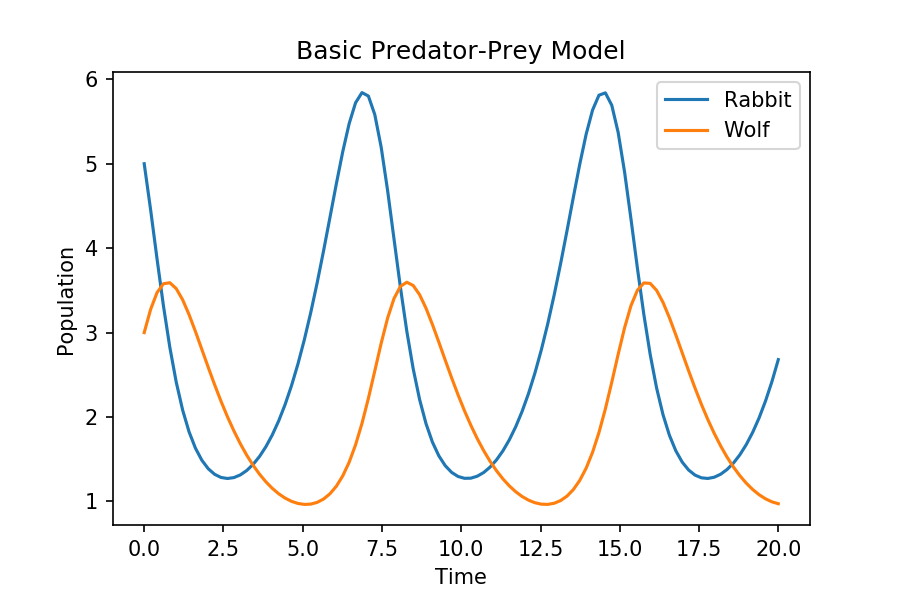
\includegraphics[width=\textwidth]{figures/Predator_Prey.png}
\caption{The solution to Problem \ref{prob:predator-prey-2} of the system found in \eqref{eqn: Pred-Prey}}
\label{fig: Pred-Prey}
\end{figure}


\begin{problem}\label{prob:predator-prey-1}
Define the function \li{predator_prey()} that accepts the current time $t$, the current $r(t)$ and $w(t)$ values as a 1d array $y$, and the parameters $\alpha, \beta, \delta$, and $\gamma$,
and returns the right hand side of \eqref{eqn: Pred-Prey} as a tuple. 
\end{problem}

\begin{problem}\label{prob:predator-prey-2}
Use \li{solve_ivp} and your function from Problem \ref{prob:predator-prey-1} to solve \eqref{eqn: Pred-Prey} with initial conditions $(r_0, w_0) = (5, 3)$ and time ranging from $0$ to $20$ years.
Use $\alpha=1.0$, $\beta=0.5$, $\delta=0.75$, and $\gamma=0.25$ as your growth parameters.
Display the resulting rabbit and wolf populations over time on the same plot. Your graph should match the graph in Figure \ref{fig: Pred-Prey}.

To pass parameters into your ODE function, use the \li{args} argument of \li{solve_ivp}. For example:
\begin{lstlisting}
# Pass the arguments into solve_ivp here:
t = np.linspace(t0, tf, t_steps)
solve_ivp(predator_prey, t_span, y0, t_eval=t,
				args=(alpha, beta, gamma, delta))
\end{lstlisting}
The populations are stored as rows in the attribute \li{y} of the output of \li{solve_ivp}.
\end{problem}

\section*{Variations on the Predator-Prey}
\subsection*{The Lotka-Volterra model}
The representation of the predator-prey relationship found in \eqref{eqn: Pred-Prey} is called the Lotka-Volterra predator-prey model and is typically given by %. This well-known system of ODEs is typically given by
%This type of problem has a special name.
%The Lotka-Volterra predator-prey model is a well-known
%system of ODEs given by
\begin{align*}
	\frac{du}{dt} &= \alpha u - \beta uv,\\
	\frac{dv}{dt} &= -\delta v + \gamma uv.
\end{align*}
where $u$ and $v$ represent the prey and predator populations, respectively. Here $\alpha$, $\beta$, $\delta$, and $\gamma$ are the same as before but now for an arbitrary prey and predator.% represents the rate of growth of the prey, and $bu$ the amount of prey being eaten.
%Similarly, $c$ represents the rate of natural predator death, and $du$ the growth of the predator population due to the quantity of prey eaten.

The equlibria (fixed points) of a system occur when the derivatives are zero.
In this example, that occurs at $(u,v)=(0,0)$ and $(u,v)=(\frac{c}{d},\frac{a}{b})$.
%Notice also that if $v=0$ (there are no predators), the population of prey will grow exponentially.
Visualizing the phase portrait helps to give more insight into the dynamics of a system. We will do this by first nondimensionalzing our system to reduce the number of parameters.

Let $U = \frac{\gamma}{\delta}u,$ $V = \frac{\beta}{\alpha}v$, $\bar{t} = \alpha t,$ and $\eta = \frac{\gamma}{\alpha}$.
Substituting into the original ODEs we obtain the nondimensional system of equations
\begin{align}
	\begin{split}
	\frac{dU}{d\bar{t}} &= U(1-V),\\
	\frac{dV}{d\bar{t}} &= \eta V (U-1).
	\end{split}\label{lotka_volterra}
\end{align}


%\begin{figure}
%\centering
%\includegraphics[width=\textwidth]{Lotka_Volterra.pdf}
%\caption{The solution of the nondimensionalized Lotka-Volterra predator-prey equations with parameter $\alpha = 1/3$.
%This solution has initial conditions $(U,V) = (3/4, 3/4)$.}
%\label{fig: lotka-phase}
%\end{figure}

\begin{figure}[H]
\centering
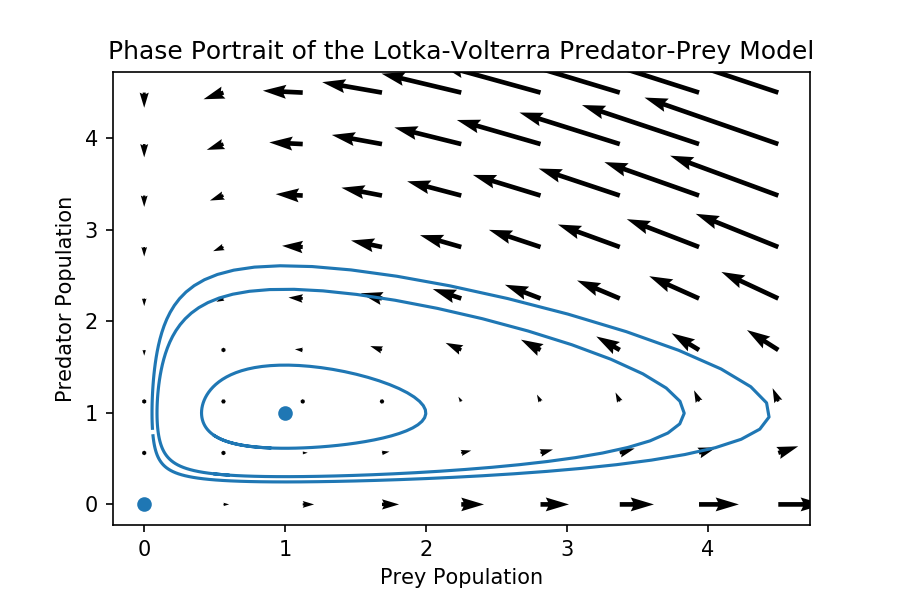
\includegraphics[width=\textwidth]{figures/LV_Phase_Portrait.png}
\caption{The phase portrait for the nondimensionalized Lotka-Volterra predator-prey equations with parameters $\eta = 1/3$.
%The portrait includes the direction field, the two equilibrium points, and the graph of the solution with initial conditions $(U,V) = (3/4, 3/4)$.
 }
\label{fig: lotka-phase}
\end{figure}

\begin{problem}
Similar to Problem \ref{prob:predator-prey-1}, define a function \li{lotka_volterra()} that takes in the current time $t$, the current predator and prey populations as a 1d array $y$, and the growth parameter $\eta$, and returns the right hand side of the nondimensional Lotka-Volterra system \eqref{lotka_volterra}.

Plot the phase portrait and several solutions of \eqref{lotka_volterra} for $\eta=1/3$.
Using \li{solve_ivp}, solve \eqref{lotka_volterra} with three different initial conditions $y_0 = (1/2, 1/3)$, $y_0=(1/2, 3/4)$, and $y_0=(1/16, 3/4)$ and time domain $t = [0,13]$. 
Plot these three solutions on the same graph as the phase portrait.
Also plot the equilibria $(0,0)$ and $(1,1)$ as points.

The following three lines of code can be used to plot the phase portrait of \eqref{lotka_volterra}:
\begin{lstlisting}
Y1, Y2 = np.meshgrid(np.linspace(0, 4.5, 9), np.linspace(0, 4.5, 9))
dU, dV = lotka_volterra(0, (Y1, Y2), eta)
Q = plt.quiver(Y1, Y2, U, V)
\end{lstlisting}

Since your solutions are being plotted with the phase portrait, plot the two populations against each other (instead of both individually against time). Your plot should match Figure \ref{fig: lotka-phase}.
\end{problem}


\subsection*{The Logistic model}
Notice that the Lotka-Volterra equations predict that prey populations will grow exponentially in the absence of predators. The logistic predator-prey equations change this dynamic by adding a carrying capacity $K$ to the prey population:
\begin{align*}
	\frac{du}{dt} &= \alpha u\left(1 -\frac{u}{K}\right) - \beta uv,\\
	\frac{dv}{dt} &= -\delta v + \gamma uv.
\end{align*}
We can again do dimensional analysis on this system to simplify parameters. Let $U = \frac{u}{K},$ $V = \frac{\beta}{\alpha}v$, $\bar{t} = \alpha t,$  $\eta = \frac{\gamma K}{\alpha}$, and $\rho = \frac{\delta}{\gamma K}$.
Then the nondimensional logistic equations are
\begin{align}
	\begin{split}
	\frac{dU}{d\bar{t}} &= U(1-U-V),\\
	\frac{dV}{d\bar{t}} &= \eta V (U-\rho).
	\end{split} \label{logistic_pred_prey}
\end{align}

\begin{problem}
Define a new function \li{logistic_model()} that takes in the current time $t$, the current predator and prey populations $y$, the parameters $\eta$ and $\rho$, and returns the right hand side of the nondimensional logistic model \eqref{logistic_pred_prey} as a tuple.

Use \li{solve_ivp} to compute solutions $(U,V)$ of \eqref{logistic_pred_prey}
for initial conditions $(1/3, 1/3)$ and $(1/2, 1/5)$ with $(t_0,t_f)=(0,13)$.
Do this for parameter values $\eta=1$, $\rho = 0.3$ and also for values $\eta=1$, $\rho = 1.1$.

Create a phase portrait for the logistic equations for each set of parameter values.
Plot the direction field, all equilibrium points, and both solution orbits on the same plot for each set of parameter values.

Hint: there are three equilibrium points for each set of parameter values.
However, you only need to plot the ones with nonnegative values of $U$ and $V$, as these are the only ones that correspond to physically-meaningful solutions.
\end{problem} 

\subsection*{Competition between Prey}
One interesting extension we can consider is what happens if we have multiple species of prey competing for the resources of their environment as well as are hunted by predators.
Supppose we now wish to model the populations of rabbits (prey), elk (also prey), and wolves in Yellowstone.
For simplicity, we will assume that the two prey populations share strictly the same resources, and can support up to either $K_1$ rabbits or $K_2$ elk.
Let $u$ be the population of rabbits, $v$ the population of elk, and $w$ the population of wolves.
Expanding on the logistic model, we can model their populations as follows:
\begin{align*}
\frac{du}{dt}&=\alpha_1 u\left(1-\frac{u}{K_1}-\frac{v}{K_2}\right)-\beta_1wu
\\
\frac{dv}{dt}&=\alpha_2 v\left(1-\frac{u}{K_1}-\frac{v}{K_2}\right)-\beta_2wv
\\
\frac{dw}{dt}&=-\delta w + \gamma_1 wu + \gamma_2 wv.
\end{align*}
We again perform dimensional analysis to reduce the number of parameters.
Let $U=\frac{u}{K_1}$, $V=\frac{v}{K_2}$, $W=\frac{\beta_1}{\alpha_1}w$, and $\bar t=\alpha_1 t$, and define new parameters as $\eta=\frac{\gamma_1K_1}{\alpha_1}$, $\rho=\frac{\delta}{\gamma_1K_1}$, $\xi=\frac{\gamma_2K_2}{\gamma_1K_1}$, $\alpha=\frac{\alpha_2}{\alpha_1}$, and $\beta=\frac{\beta_2}{\beta_1}$.
Then, the nondimensional equations for two prey species are
\begin{equation}\label{eqn:two-prey-species}
	\begin{split}
	\frac{dU}{d\overline{t}} &= U(1-U-V-W),\\
	\frac{dV}{d\overline{t}} &= \alpha V(1-U-V) - \beta VW,\\
	\frac{dW}{d\overline{t}} &= \eta W(U+\xi V-\rho).
	\end{split}
\end{equation}

\begin{problem}
Define a new function \li{two_prey_species()} that takes in the current time $t$, the current prey and predator populations $y$, the parameters $\alpha,\beta,\eta,\xi$, and $\rho$, and returns the right-hand-side of the nondimensional two prey species system \eqref{eqn:two-prey-species} as a tuple.

Use \li{solve_ivp} to compute solutions $(U,V,W)$ of \eqref{eqn:two-prey-species} using the three initial condition $(1/3,1/3,1/3)$, $(1/2,1/3,1/5)$, and $(1,1/10,1/2)$, with $(t_0,t_f)=(0,25)$.
Use parameter values $\eta=1$, $\rho=0.3$, $\xi=0.5$, $\alpha=0.2$, $\beta=0.1$.
Plot the numerical solutions for the populations as functions against time.

Do the dynamics predicted by this model seem realistic?
Write (in a markdown cell) your answer and reasoning behind it.
\end{problem}


